\documentclass[tikz,border=2pt,11pt]{standalone}
\usetikzlibrary{arrows.meta}
\usetikzlibrary{positioning}
\usepackage{amsmath}
\usepackage{amssymb}
\usepackage{tikz}
\usepackage{xcolor}
\def\@captype{figure}
\DeclareMathOperator{\Hom}{Hom}
\DeclareMathOperator{\Mod}{Mod}
\DeclareMathOperator{\sk}{sk}
\DeclareMathOperator*{\colim}{colim}
\newcommand{\id}{\mathrm{id}}
\newcommand{\sSet}{\mathbf{sSet}}
\newcommand{\Spaces}{\mathbf{Spaces}}
\newcommand{\op}{\mathrm{op}}
\newcommand{\LL}{\mathbf L}
\begin{document}
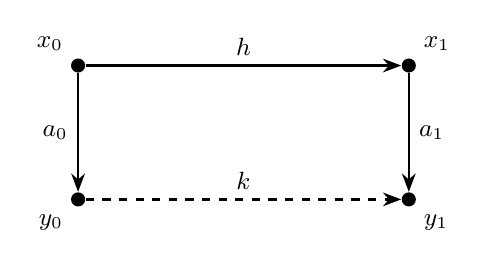
\begin{tikzpicture}[>=Stealth,
    vertex/.style={circle,fill=black,inner sep=1.8pt},
    every node/.style={font=\small}]
\node[vertex,label=above left:\(x_0\)] (x0) at (0,1.7) {};
\node[vertex,label=above right:\(x_1\)] (x1) at (4.2,1.7) {};
\node[vertex,label=below left:\(y_0\)] (y0) at (0,0) {};
\node[vertex,label=below right:\(y_1\)] (y1) at (4.2,0) {};
\draw[->,thick] (x0) -- node[above] {\(h\)} (x1);
\draw[->,thick] (x0) -- node[left] {\(a_0\)} (y0);
\draw[->,thick] (x1) -- node[right] {\(a_1\)} (y1);
\draw[->,thick,dashed] (y0) -- node[above] {\(k\)} (y1);
\end{tikzpicture}
\end{document}
